\documentclass{beamer}
\mode<presentation>{
  \usetheme{Madrid} 
}
\usepackage{pstricks}
\usepackage{listings}
\usepackage{graphicx} % Allows including images
\usepackage{booktabs} % Allows the use of \toprule, \midrule and \bottomrule in tables
\usepackage{color}

\makeatletter
\def\th@mystyle{%
    \normalfont % body font
    \setbeamercolor{block title example}{bg=orange,fg=white}
    \setbeamercolor{block body example}{bg=orange!20,fg=black}
    \def\inserttheoremblockenv{exampleblock}
  }
\makeatother
\theoremstyle{mystyle}
\newtheorem*{attention}{Attention !!!}

\title{Ruby on Rails training}
\author{Wojtek Sykurski}
\institute[Samsung R\&D]
{
  Samsung R\&D Poland \\
  \medskip
  \textit{w.sykurski@samsung.com}
}
\date{\today}

\begin{document}
\defverbatim[colored]\newappGI{
  \begin{lstlisting}[language=bash,basicstyle=\ttfamily,
    keywordstyle=\color{red}]
   mkdir Rails_Group_1 
   cd Rails_Group_1
   rails new helldesk
   rails server
  \end{lstlisting}
}

\defverbatim[colored]\newappGII{
  \begin{lstlisting}[language=bash,basicstyle=\ttfamily,
    keywordstyle=\color{red}]
   mkdir Rails_Group_2 
   cd Rails_Group_2
   rails new helldesk
   rails server
  \end{lstlisting}
}


\defverbatim[colored]\newappworking{
  \begin{lstlisting}[language=bash,basicstyle=\ttfamily,
    keywordstyle=\color{red}]
   mkdir Rails_Group_2 
   cd Rails_Group_2
   rails new helldesk
   bundle install
   rails server
  \end{lstlisting}
}

\defverbatim[colored]\modelexample{
  \begin{lstlisting}[language=ruby,basicstyle=\ttfamily,
    keywordstyle=\color{red}]
    class User < ActiveRecord::Base
      validates :name, :presence => true,
                :uniqueness => true
      validates :password, :confirmation => true
      ...
    end
\end{lstlisting}
}

\defverbatim[colored]\viewexample{
  \begin{lstlisting}[language=ruby,basicstyle=\tiny,
    keywordstyle=\color{red}]
<% provide(:title, 'Index') %>
<h1>Listing Users</h1>
<% if notice %>
  <p id="notice"><%= notice %></p>
<% end %>
<table>
<tbody>
    <% @users.each do |user| %>
      <tr>
        <td><%= user.name %></td>
        <td><%= user.email %></td>
        <div class="actions">
            <td><%= link_to 'Show', user %></td>
            <td><%= link_to 'Edit', edit_user_path(user) %></td>
            <td><%= link_to 'Destroy', user, method: :delete, data: { confirm: 'Are you sure?' } %></td>
        </div>
      </tr>
    <% end %>
  </tbody>
</table>
<br>
<%= link_to 'New User', new_user_path %>
\end{lstlisting}
}

\defverbatim[colored]\classexample{
  \begin{lstlisting}[language=ruby,basicstyle=\tiny,
    keywordstyle=\color{red}]
    class TestClass
       def initialize
         @instance_var=10
       end

       def method
         put 'I am test class'
       end

       def instance_var
         return @instance_var
       end

       def instance_var=(var)
         @instance_var = var
       end
    end
\end{lstlisting}
}


\defverbatim[colored]\classexampleII{
  \begin{lstlisting}[language=ruby,basicstyle=\small,
    keywordstyle=\color{red}]
    class TestClass
       attr_accessor :instance_var
       def initialize
         @instance_var=10
       end

       def method
         put 'I am test class'
       end

    end
\end{lstlisting}
}

\defverbatim[colored]\classexampleprivateI{
  \begin{lstlisting}[language=ruby,basicstyle=\tiny,
    keywordstyle=\color{red}]
    class TestClass
       attr_accessor :instance_var
       def initialize
         @instance_var=10
         method
       end
       
       private:

       def method
         put 'I am test class'
       end

    end
\end{lstlisting}
}

\defverbatim[colored]\classexampleprivateII{
  \begin{lstlisting}[language=ruby,basicstyle=\tiny,
    keywordstyle=\color{red}]
    class TestClass
       attr_accessor :instance_var
       def initialize
         @instance_var=10
         method
       end

       def method1
         put 'I am test class'
       end
       
       def method2
         put 'I am test class'
       end

       private :method, :method2

    end
\end{lstlisting}
}

\defverbatim[colored]\classexampleprotected{
  \begin{lstlisting}[language=ruby,basicstyle=\tiny,
    keywordstyle=\color{red}]
    class TestClass
       attr_accessor :instance_var
       def initialize
         @instance_var=10
         method
       end

       protected:

       def method1
         put 'I am test class'
       end
       
       def method2
         put 'I am test class'
       end
    end
\end{lstlisting}
}

\defverbatim[colored]\railsgenerator{
  \begin{lstlisting}[language=bash,basicstyle=\tiny,
    keywordstyle=\color{red}]
    rails generate controller static_content start about help
\end{lstlisting}
}

\defverbatim[colored]\railschangeroute{
  \begin{lstlisting}[language=bash,basicstyle=\small,
    keywordstyle=\color{red}]
    root 'static_content#start'
\end{lstlisting}
}

\defverbatim[colored]\railstopmenu{
  \begin{lstlisting}[language=ruby,basicstyle=\tiny,
    keywordstyle=\color{red}]
    <div id="left_menu">
        <ul>
            <li> <%= link_to "Issues", "#" %> </li>
            <li> <%= link_to "Admin", "#" %> </li>
        </ul> 
    </div>

    <div>
        <ul>
            <li> <%= link_to "Login", "#" %></li>
            <li> <%= link_to "About", "#" %></li>
            <li> <%= link_to "Help", "#" %></li>
        </ul>
    </div>
\end{lstlisting}
}


\defverbatim[colored]\railspartial{
  \begin{lstlisting}[language=ruby,basicstyle=\small,
    keywordstyle=\color{red}]
    <%= redren 'layouts/top_menu" %>
\end{lstlisting}
}

\defverbatim[colored]\railsprovide{
  \begin{lstlisting}[language=ruby,basicstyle=\small,
    keywordstyle=\color{red}]
    <% provide(:title, 'Index') %> 
\end{lstlisting}
}

\defverbatim[colored]\railslayouthandletitle{
  \begin{lstlisting}[language=ruby,basicstyle=\small,
    keywordstyle=\color{red}]
    <% unless yield(:title).empty? %> 
        <title>Helldesk2 | <%=yield(:title)%> </title> 
    <%else %>
        <title>Helldesk2</title> 
    <% end %> 
\end{lstlisting}
}


\defverbatim[colored]\railshelperI{
  \begin{lstlisting}[language=ruby,basicstyle=\tiny,
    keywordstyle=\color{red}]
    def provide_title(subtitle='')
     hell = "Helldesk"
     if subtitle.empty?
       hell
     else
       hell + " | " + subtitle
    end
  end

\end{lstlisting}
}

\defverbatim[colored]\routeupdateI{
  \begin{lstlisting}[language=ruby,basicstyle=\tiny,
    keywordstyle=\color{red}]
    controller :static_content do
       get 'start' => :start
       get 'help' => :help
       get 'about' => :about
    end

\end{lstlisting}
}



\defverbatim[colored]\railstitlehelperinlayout{
  \begin{lstlisting}[language=ruby,basicstyle=\small,
    keywordstyle=\color{red}]
    <title><%=provide_title(yield(:title))%></title>

\end{lstlisting}
}

\defverbatim[colored]\generatorscaffold{
  \begin{lstlisting}[language=bash,basicstyle=\tiny,
    keywordstyle=\color{red}]
    rails generate scaffold User name:string email:string hash_password:string salt:string
\end{lstlisting}
}

\defverbatim[colored]\databasemigrationuser{
  \begin{lstlisting}[language=bash,basicstyle=\small,
    keywordstyle=\color{red}]
    rake db:migrate
\end{lstlisting}
}

\defverbatim[colored]\railsreallinksI{
  \begin{lstlisting}[language=html,basicstyle=\tiny,
    keywordstyle=\color{red}]
    <div id="right_menu">
        <ul>
            <li> <%= link_to "Login", "#" %></li>
            <li> <%= link_to "About", :about %></li>
            <li> <%= link_to "Help", :help %></li>
        </ul>
    </div> 

\end{lstlisting}
}


\defverbatim[colored]\migrationuser{
  \begin{lstlisting}[language=ruby,basicstyle=\tiny,
    keywordstyle=\color{red}]
    class CreateUsers < ActiveRecord::Migration
    def change
     create_table :users do |t|
       t.string :name
       t.string :email
       t.string :hash_password
       t.string :salt

       t.timestamps null: false
      end
     end
    end  

\end{lstlisting}
}


\defverbatim[colored]\railsconsolestart{
  \begin{lstlisting}[language=ruby,basicstyle=\small,
    keywordstyle=\color{red}]
    rails console development
\end{lstlisting}
}

\defverbatim[colored]\railsimportsha{
  \begin{lstlisting}[language=ruby,basicstyle=\small,
    keywordstyle=\color{red}]
    require 'digest/sha2' 
\end{lstlisting}
}

\defverbatim[colored]\railsconsoleencrypt{
  \begin{lstlisting}[language=ruby,basicstyle=\small,
    keywordstyle=\color{red}]
    Digest::SHA2.hexdigest(``example_word'')
\end{lstlisting}
}

\defverbatim[colored]\railsusermodelI{
  \begin{lstlisting}[language=ruby,basicstyle=\tiny,
    keywordstyle=\color{red}]
    class User < ActiveRecord::Base
      validates :name, :presence => true, :uniqueness => true

\end{lstlisting}
}

\defverbatim[colored]\railsusermodelII{
  \begin{lstlisting}[language=ruby,basicstyle=\tiny,
    keywordstyle=\color{red}]
    require 'digest/sha2'
    class User < ActiveRecord::Base
      validates :name, :presence => true, :uniqueness => true
      validates :password, :confirmation => true
      attr_accessor :password_confirmation
      attr_reader :password
      validate :password_must_be_present

      def User.encrypt_password(password, salt)
        Digest::SHA2.hexdigest(password + "slowo" + salt) 
      end

      def password=(password)
        @password = password
        if password.present?
          generate_salt
          self.hash_password = self.class.encrypt_password(password,self.salt)
        end
      end

      def User.authenticate(name,password)
        if user = User.find_by_name(name)
          if user.hash_password == encrypt_password(password, user.salt)
            user
          end
        end
      end

\end{lstlisting}
}

\defverbatim[colored]\railsusermodelIII{
  \begin{lstlisting}[language=ruby,basicstyle=\tiny,
    keywordstyle=\color{red}]
      private

      def password_must_be_present
        errors.add(:password, "Missing password") unless hash_password.present?
      end

      def generate_salt
        self.salt = self.object_id.to_s + rand.to_s
      end
    end
\end{lstlisting}
}


\defverbatim[colored]\railsusercontroller{
  \begin{lstlisting}[language=ruby,basicstyle=\tiny,
    keywordstyle=\color{red}]
    # Never trust parameters from the scary internet, only allow the white list through.
    def user_params
      params.require(:user).permit(:name, :email, :password, :password_confirmation)
    end 
\end{lstlisting}
}

\defverbatim[colored]\railsuserviewform{
  \begin{lstlisting}[language=ruby,basicstyle=\tiny,
    keywordstyle=\color{red}]
  <div class="field">
    <%= f.label :name %><br>
    <%= f.text_field :name %>
  </div>
  <div class="field">
    <%= f.label :email %><br>
    <%= f.text_field :email %>
  </div>
  <div class="field">
    <%= f.label :password %><br>
    <%= f.password_field :password %>
  </div>
  <div class="field">
    <%= f.label :password_confirmation %><br>
    <%= f.password_field :password_confirmation %>
  </div>
  <div class="actions">
    <%= f.submit %>
  </div>

\end{lstlisting}
}


\begin{frame}
  \titlepage 
\end{frame}

\begin{frame}
  \frametitle{Agenda}
  \tableofcontents[hideallsubsections]
\end{frame}

\section{First Day: Introduction \& (mostly) Static Content}
\begin{frame}
  \frametitle{Day First Agenda:}
  \tableofcontents
  [
  currentsection,
  sectionstyle=hide/hide,
  subsectionstyle=show/show/hide
  ]
\end{frame}

\subsection{Web Applications Frameworks}

\begin{frame}
  \frametitle{Technologies}
  \begin{itemize}
    \item M\$ Technologies
    \item Rest of the World
  \end{itemize}
  
\end{frame}

\subsection{Technologies}

    \subsubsection{Most popular}

    \begin{frame}
      \frametitle{Technologies - Rest of the world}
      \begin{itemize}
        \item Pure HTML
        \item Java - different technologies
        \item PHP
        \item Python based Frameworks
          \begin{itemize}
            \item Django
            \item web2py
            \item TurboGears
            \item Others
          \end{itemize}
        \item Ruby based Frameworks
          \begin{itemize}
            \item Ruby on Rails
            \item Sinatra
            \item Cuba, Merb and many others
          \end{itemize}
      \end{itemize}

    \end{frame}


    \subsubsection{Ruby on Rails}

    \begin{frame}
      \frametitle{Technologies - Ruby on Rails}
      \begin{itemize}
        \item Fully operational Web Framework:
          \begin{itemize}
            \item Build in WebServer(Webrick)
            \item Database Engine (SQLight)
            \item Debuging and Tracking tools
            \item Support for plugins:
              \begin{itemize}
                \item Made ``by hand''
                \item Ruby Gems 
              \end{itemize}

          \end{itemize}
        \item Use MCV model
          \begin{itemize}
            \item Model - Database communication
            \item View - User Front-end
            \item Controller - Integration and synchronization between Model and View
          \end{itemize}
        \item Integration with most of popular Web servers and Databases

      \end{itemize}

    \end{frame}

\subsection{Ruby}
\begin{frame}
  \frametitle{Ruby}
  \begin{itemize}
    \item High level programming language
      \begin{itemize}
        \item Dynamic \& Reflective
          \begin{itemize}
            \item ``On Fly'' Compilation and execution
            \item Drawback - errors handling and detection
            \item ``Test driven development''
          \end{itemize}
        \item Object orientated
      \end{itemize}
    \item Similar to python
    \item Interactive shell - irb
\end{itemize}
\end{frame}

\begin{frame}
  \frametitle{Ruby - Interactive Shell }
  Starting IRB:
  \begin{itemize}
    \item Start terminal
    \item Type ``irb''
  \end{itemize}
\end{frame}

\begin{frame}
  \frametitle{Ruby - variables}
    \begin{definition}
      Global Variables - sporadic use in Ruby on Rails:
    \end{definition}
    \begin{example}
      $ \$Global\_Var=10$
    \end{example}
  \begin{itemize}
    \item Instance Variables - very often used in Ruby on Rails:
      \begin{itemize}
        \item $ @Instance\_Var=10$
        \item RoR usage - transfer data between controller, model and view
      \end{itemize}
    \item Class Variables - in practice - never used in RoR:
      \begin{itemize}
        \item $ @@Class\_Var=10$
      \end{itemize}
    \item Local Variables - common use in RoR:
      \begin{itemize}
        \item $ Local\_Var=10$
      \end{itemize}
    \end{itemize}
  
\end{frame}

\begin{frame}
  \frametitle{Ruby - operators}
  \begin{itemize}
    \item Add, Sub, Multiply, Divide, Power
      \begin{itemize}
        \item numbers
        \item $var1=3*3$
        \item $var1**3$
        \item string, some other classes
        \item $var2 = 'jakis tekst '$
        \item $var2 * 3$
      \end{itemize}
    \item Assign value
      \begin{itemize}
        \item Standard operators
        \item Ruby special
      \end{itemize}
  \end{itemize}
  
\end{frame}

\begin{frame}
  \frametitle{Ruby - classes}
  \begin{definition}[Class]
    Class is a template for custom objects creation. Those objects contains
    member variables and functions (methods)
  \end{definition}
  \classexample
  
\end{frame}

\begin{frame}
  \frametitle{Ruby - classes - attribute accessor}
  \begin{definition}[Attribute Accessor]
    Attribute accessor provide easy access to instance variables
  \end{definition}
  \classexampleII
\end{frame}

\begin{frame}
  \frametitle{Ruby - classes - private/protected}
  \begin{definition}[Private methods]
    Private methods - can only be used by other methods of the same object.
    \textcolor{red}{AND OBJECT OF CLASSES that inherit from this class !!!}
  \end{definition}

  \classexampleprivateI

\end{frame}

\begin{frame}
  \frametitle{Ruby - classes - private/protected}
  \begin{definition}[Private methods]
    Private methods - different annotation.
  \end{definition}

  \classexampleprivateII

\end{frame}

\begin{frame}
  \frametitle{Ruby - classes - protected}
  \begin{definition}[Protected]
    Protected works almost the same way as private!\\*
    \textcolor{red}{Only difference is that protected methods can be used by other objects of the same class}
  \end{definition}
  
  \classexampleprotected
\end{frame}

\begin{frame}
  \frametitle{Ruby - gems}
  \begin{definition}
    Ruby gems - packs of plugins, libraries, binaries and source code files,
    which can be fast added to our existing Ruby projects. It is similar to
    Python \textcolor{blue}{pip} tool.
  \end{definition}
  
  \begin{definition}
    In Ruby on Rails gem's handling is done by tool called ``bundler''.
  \end{definition}
  
  \begin{example}
    Popular RoR gems:
    \begin{itemize}
    \item \textcolor{blue}{Carrier}
    \item \textcolor{blue}{Authlogic}
    \item \textcolor{blue}{RMagic}
    \item \textcolor{blue}{Sass} - present by default in RoR from version 3
    \end{itemize}
  \end{example}
\end{frame} 

\subsection{Ruby on Rails}

\subsubsection{Fast Start}
\begin{frame}
  \frametitle{Ruby on Rails - fast start}
  \newappGI
  \newappGII
\end{frame}

\begin{frame}
  \frametitle{Ruby on Rails - install gems to environment}
  \begin{definition}
    Bundler - we need to use it, after creating new app. It would install all
    required gems and libraries in our environment. On most of systems it will
    start automatic after creating new app. If not, just run:\\*
    bundle install
  \end{definition}
  Now, go for http address:
  \textcolor{red}{http://localhost:3000}
\end{frame}

\begin{frame}
  \frametitle{Ruby on Rails - structure}
  Main components of RoR application:
  \begin{itemize}
  \item MCV model
  \item Configuration
    \begin{itemize}
      \item Environments
      \item Database
      \item Gemfile
      \item Routes
    \end{itemize}
  \item Utils
    \begin{itemize}
      \item Routes
      \item Rake
      \item Bundler
    \end{itemize}
  \end{itemize}
  
\end{frame}

\subsubsection{MCV}
\begin{frame}
  \frametitle{Ruby on Rails - MCV }
  \begin{definition}
    MCV (Model, Controller, View) is a software architecture used in RoR.
    It separates database operations (Model), content generation (View)
    and application logic (Controller) in to different components.
  \end{definition}
  \begin{figure}[h]
   \centering
      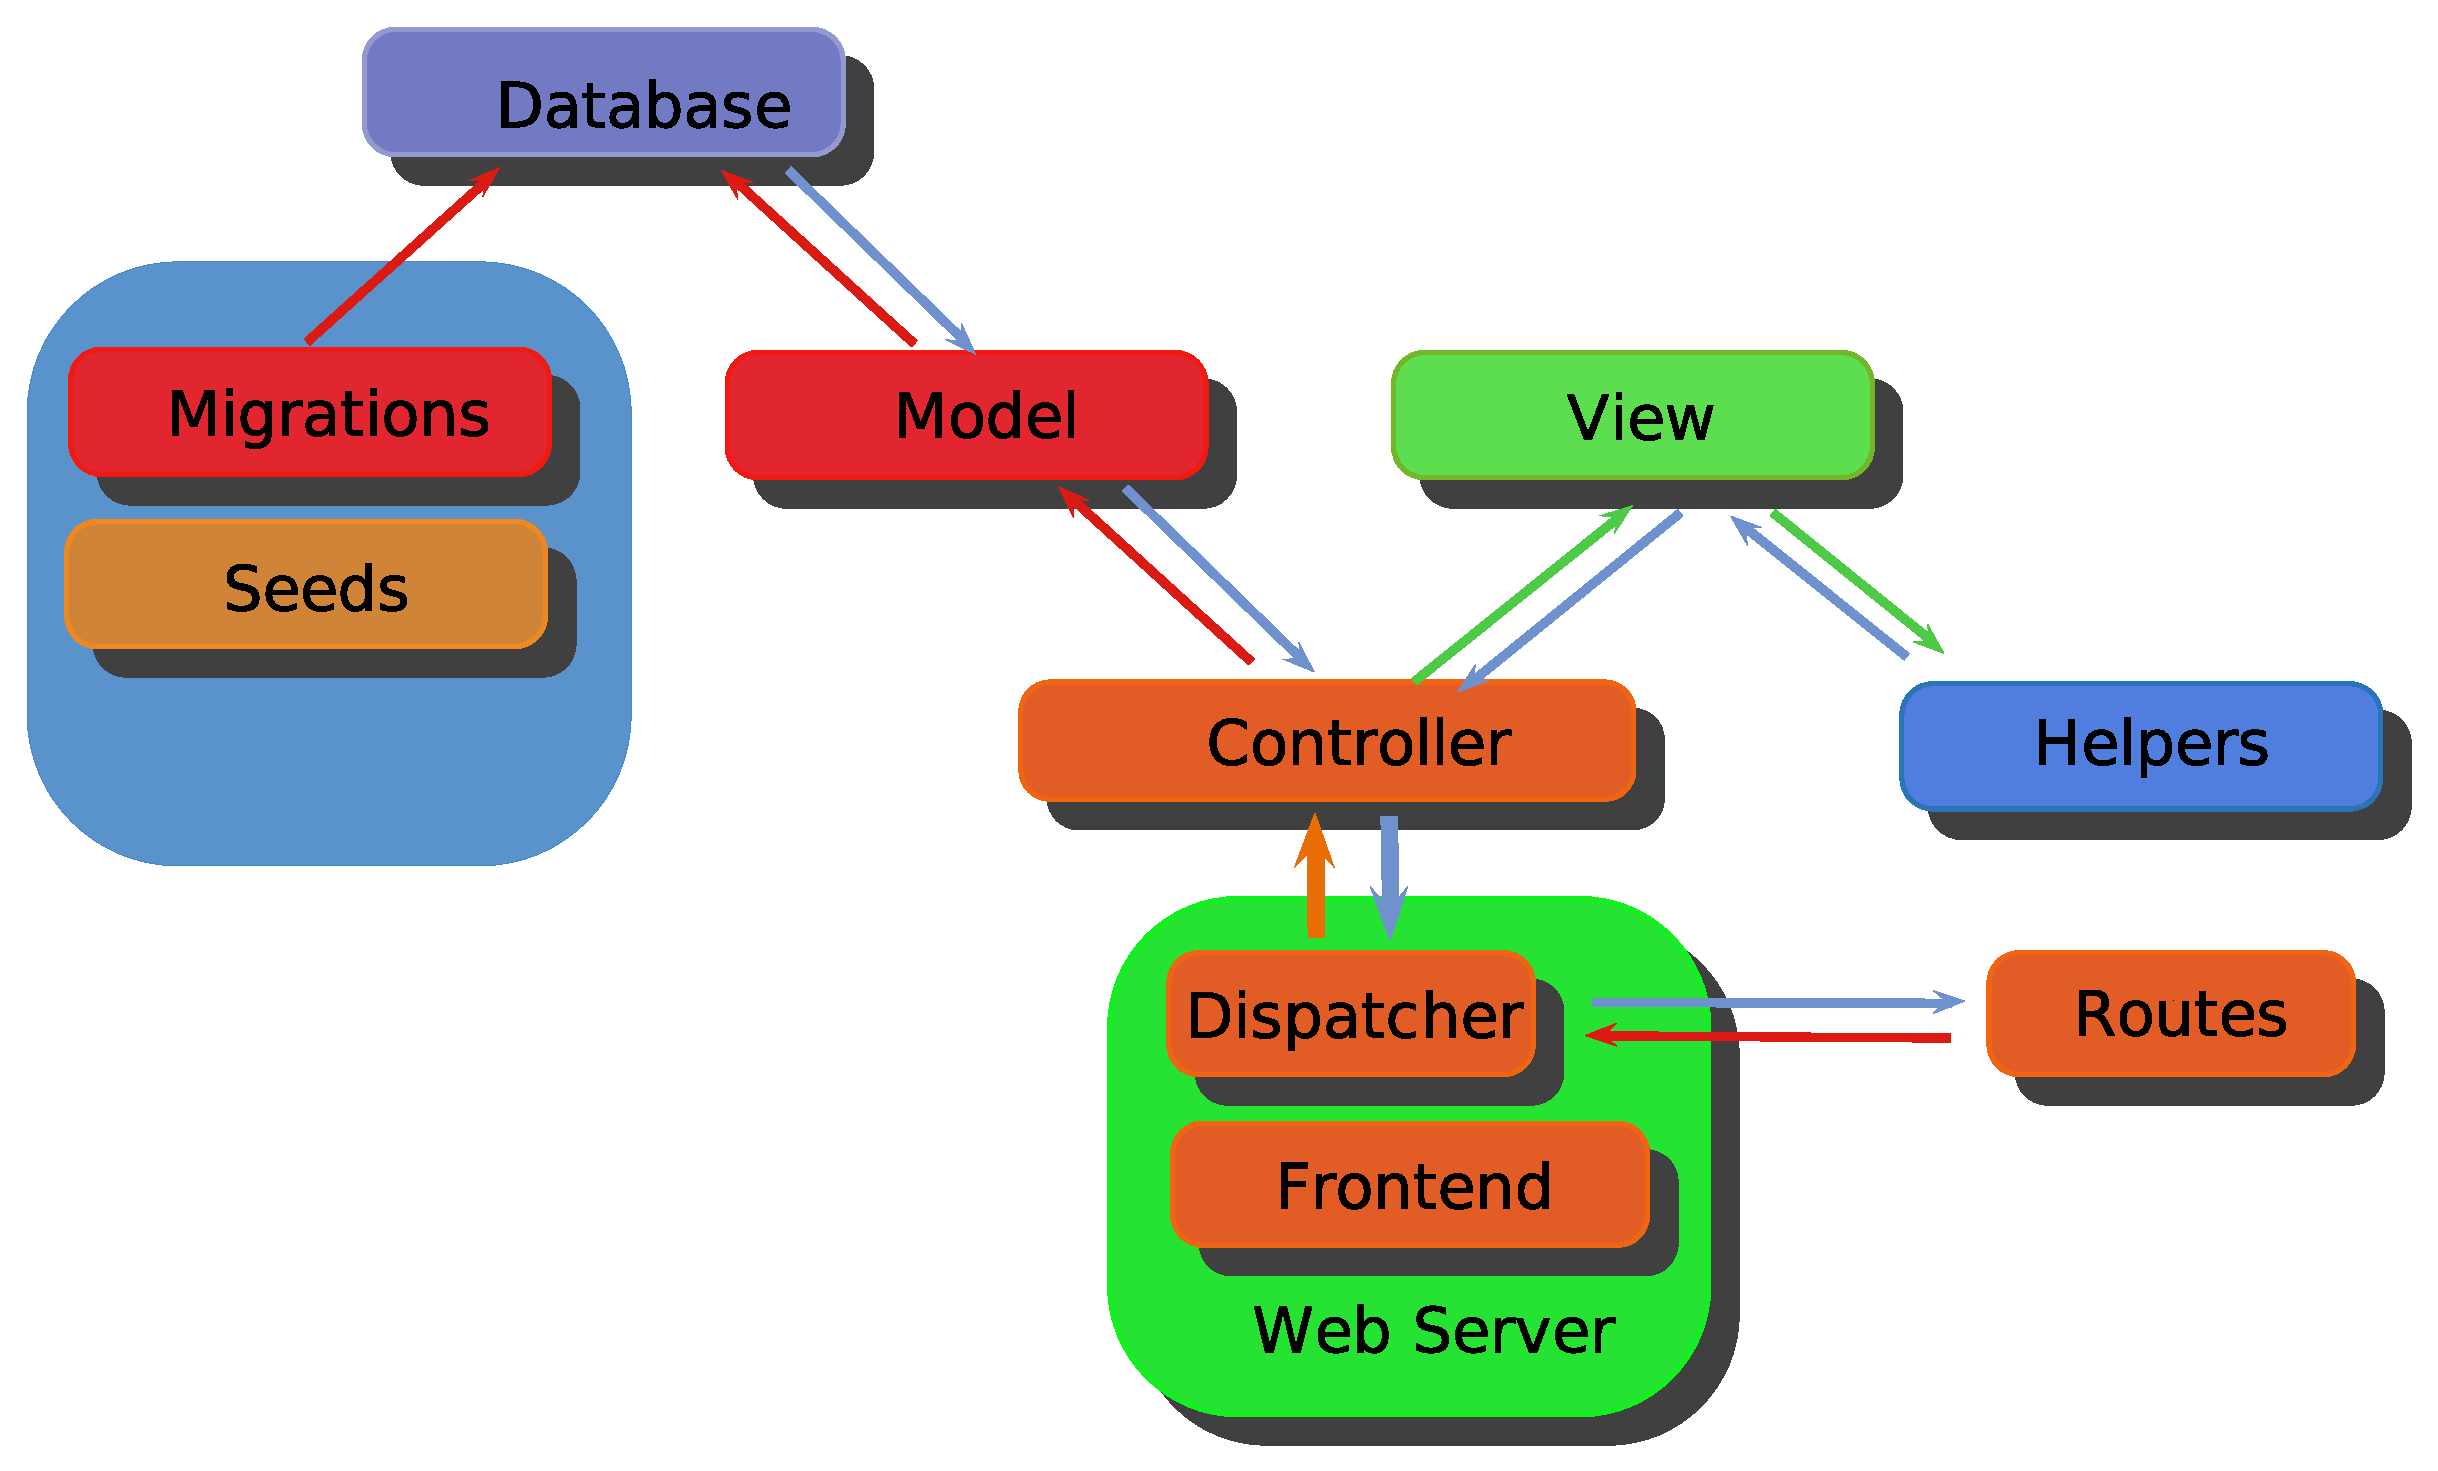
\includegraphics[width = 0.7\textwidth]{./mcv1.eps}
  \end{figure}
  
\end{frame}

\begin{frame}
  \frametitle{Ruby on Rails - Model}
  \begin{definition}
    Model - describes database object (usual table), relations with other
    models and validations of data.
  \end{definition}
  \begin{example}[user.rb]
    \modelexample
  \end{example}
  \begin{attention}
    \alert{Models DO NOT} describe table structure, column names, data types and so.
  \end{attention}
\end{frame}

\begin{frame}
  \frametitle{Ruby on Rails - controller}
  \begin{definition}
    Controller is responsible for application logic by providing connection
    between models, views, libraries and gems.
    It handles and generates requests from web server.
  \end{definition}
  
\end{frame}

\begin{frame}
  \frametitle{Ruby on Rails - View}
  How does Rails generate page:
  \begin{columns}
    \begin{column}{0.5\textwidth}
      Main elements:
      \begin{itemize}
        \item Layout
        \item View
        \item Partial 
      \end{itemize}
      Other:
      \begin{itemize}
        \item Helpers 
        \item Assets 
          \begin{itemize}
            \item js, coffee scrpits
            \item css
            \item images, video, music, etc.
          \end{itemize}
      \end{itemize}
    \end{column}
    
    \begin{column}{0.5\textwidth}
      \begin{figure}[h]
        \centering 
        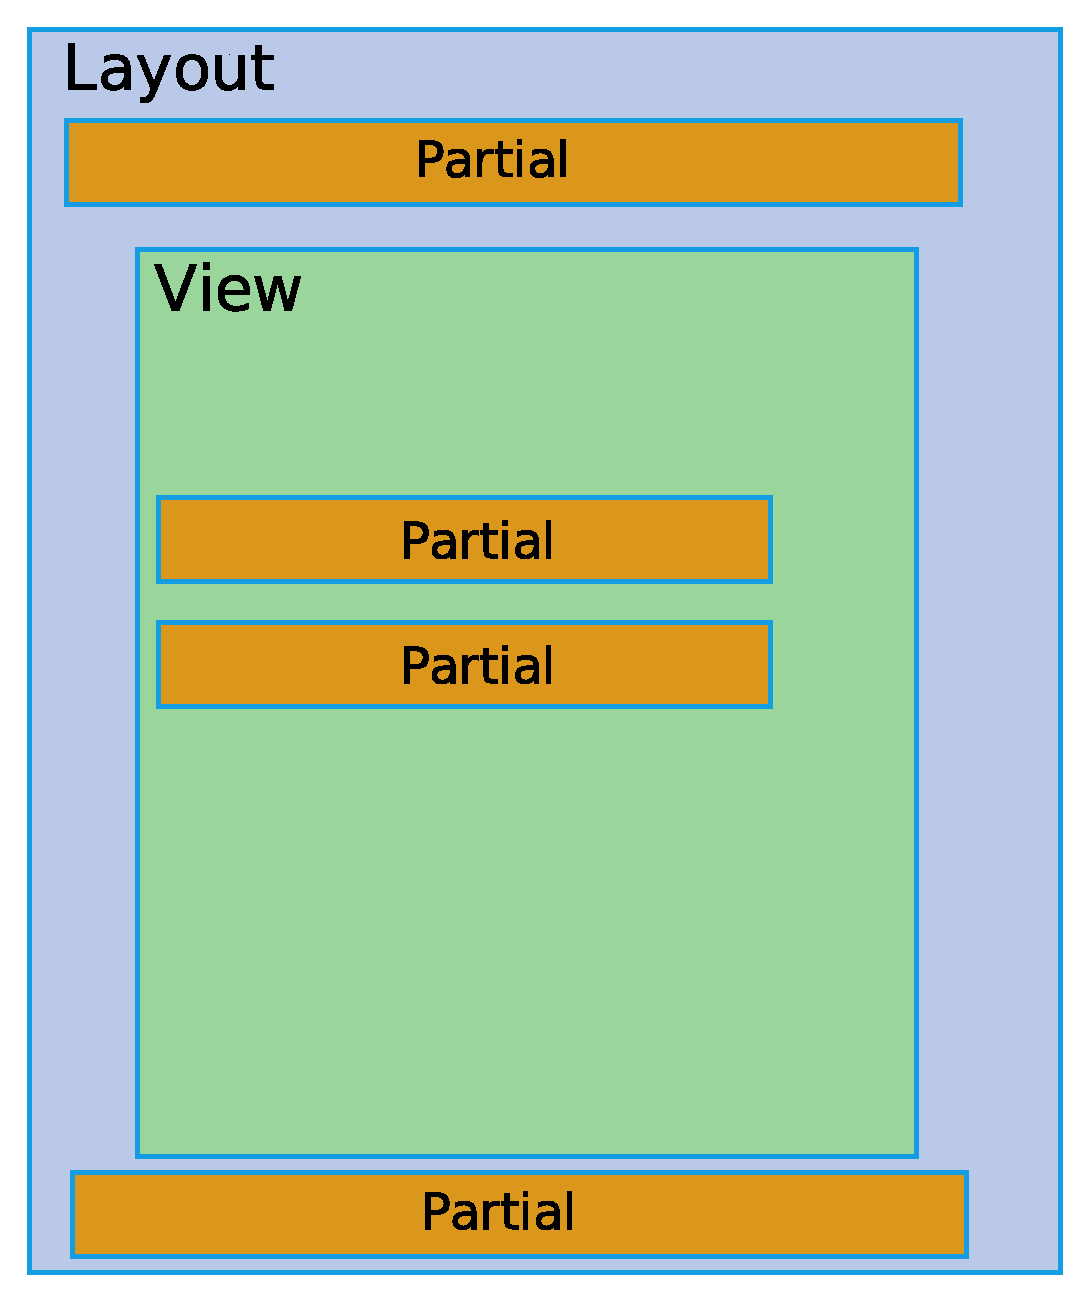
\includegraphics[width = 0.7\textwidth]{./Layout_view_partial.eps}
      \end{figure}
    \end{column}
  \end{columns}
  
\end{frame}

\begin{frame}
  \frametitle{Ruby on Rails - View}
  \begin{definition}
    View contains the html web page structure, with additional RoR logic
  \end{definition}
  \begin{example}[user.html.erb]
    \viewexample
  \end{example}
\end{frame}

\begin{frame}
  \frametitle{Ruby on Rails - View Layout}
  \begin{definition}{Layout}
    Layout contain general structure of page. 
    Views are generated ``inside'' application layout file
  \end{definition}
  \begin{example}[user.html.erb]
    \viewexample
  \end{example}
\end{frame}

\begin{frame}
  \frametitle{Ruby on Rails - Environments}
  \begin{definition}{RoR Environments}
      Environments - describes server run time environment, can be used for other
      configuration files.
  \end{definition}
  Files:
  \begin{itemize}
  \item All files in ./config/environments
  \item ./config/environments.rb
  \end{itemize}
  \begin{example}
    \begin{itemize}
    \item Development - will be used during this course
    \item Production - will be used during this course
    \item Test - will be used during this course
    \end{itemize}
  \end{example}
  
\end{frame}

\begin{frame}
  \frametitle{Ruby on Rails - Create basic content}
  \begin{definition}
    Rails generator - tool for controllers, views, models and helpers automatic creation
  \end{definition}
  For now, lets just put this in terminal:
  \railsgenerator
  And go to:\\*
  \textcolor{red}{http://localhost:3000/static\_content/start}
  \textcolor{red}{http://localhost:3000/static\_content/about}
  \textcolor{red}{http://localhost:3000/static\_content/help}
  
\end{frame}

\begin{frame}
  \frametitle{Ruby on Rails - Change page root}
  \begin{definition}
    Rails routes describes how to redirect html requests to specific controller/view
    File location: ./config/routes.rb
  \end{definition}
  To change Web app root to specific controller and view, add following to this file:
  \railschangeroute
\end{frame}

\subsection{Layouts}
\begin{frame}
  \frametitle{Customizing layout }
  \begin{columns}
    \begin{column}{0.5\textwidth}
      What we want to achieve:
      \begin{figure}[h]
      \centering
       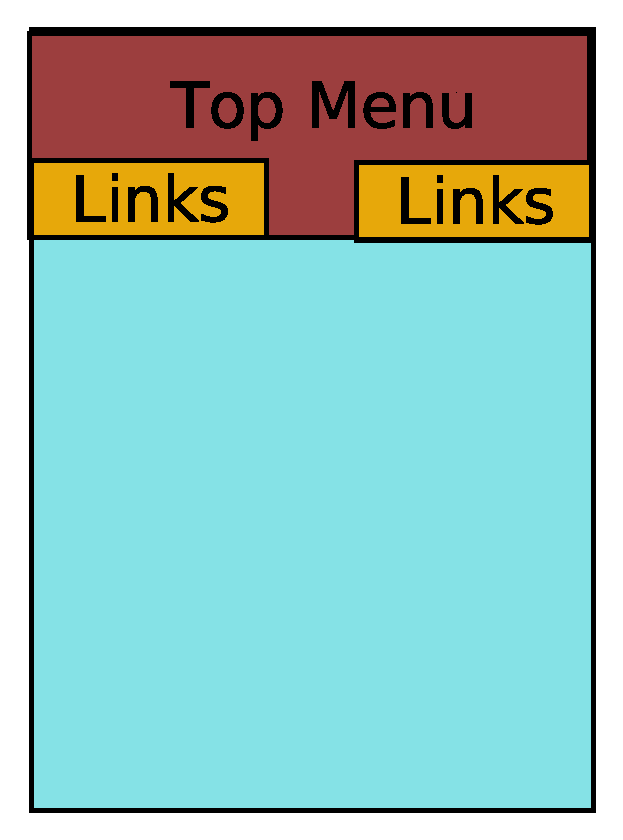
\includegraphics[width = 0.7\textwidth]{./page_layout.eps}
      \end{figure}
    \end{column}
    \begin{column}{0.5\textwidth}

          Required Steps:
          \begin{itemize}
          \item Add top menu:
            \begin{itemize}
            \item List of links
            \item Custom CSS with positioning
            \end{itemize}
          \item Display top menu on all pages
            \begin{itemize}
              \item Needs to be added to Layout
              \item Use of ``Partials''
            \end{itemize}
          \item Dynamic Pages Title generation
            \begin{itemize}
              \item Provide title for every subpage
              \item Error handling if subpage has none
              \item Create custom functions for handling all those conditions
              \item Place theme in helper
            \end{itemize}

          \end{itemize}
    \end{column}
  \end{columns}
\end{frame}

\begin{frame}
  \frametitle{Layouts - Creating top menu}
  Add folowing code to ./app/views/layouts/application.html.erb in ``Body''
  section:
  \railstopmenu
  
\end{frame}

\begin{frame}
  \frametitle{Layouts - Customizing CSS}
  \begin{itemize}
    \item Display links in line 
    \item Left and Right menu
    \item Place menu on top
    \item Add some CSS3 effects - useful link: http://www.css3maker.com/
  \end{itemize}
  
\end{frame}

\begin{frame}
  \frametitle{Layouts - Move top menu to Partial}
  \begin{definition}
    Partial is fragment of HTML code which can be included in other Web Pages.
    It is very useful for generating lists, tables (for ex. table of products)
    and navigation menus 
  \end{definition}
  In this case, We want to move source code from application layout to partial,
  to make it more clean and readable.
  Required steps:
  \begin{itemize}
    \item Create new file ./app/views/layouts/\_top\_menu.html.erb
    \item Copy all top menu div to that file
    \item In application layout add \railspartial
  \end{itemize}

\end{frame}

\begin{frame}
  \frametitle{Page Title - dynamic generated}
  \begin{definition}
    To send some variable from View to Layout use the ``provide'' build in function. 
  \end{definition}
  \railsprovide
  To handle it in layout, following code can be used:
  \railslayouthandletitle
\end{frame}

\begin{frame}
  \frametitle{Dynamic Title: Use Helper}
  \begin{definition}
    Helpers all special files, which behave like libraries - they store
    functions (helpers), which can be then use in views and layouts, 
    \textcolor{red}{but Not in Controllers and Models !!!}
  \end{definition}
  \railshelperI
  To call it in application layout:
  \railstitlehelperinlayout
\end{frame}


\section{Second Day: User Scaffold}
    \begin{frame}
      \frametitle{Second Day Agenda:}
      \tableofcontents
      [
      currentsection,
      sectionstyle=hide/hide,
      subsectionstyle=show/show/hide
      ]
    \end{frame}

  \subsection{What we need for User ?}
    \begin{frame}
      \frametitle{User requirements}
    \end{frame}

\section{Third Day: Loging in Application}
    \begin{frame}
      \frametitle{Third Day Agenda:}
      \tableofcontents
      [
      currentsection,
      sectionstyle=hide/hide,
      subsectionstyle=show/show/hide
      ]
    \end{frame}
  \subsection{Session}
    \begin{frame}
      \frametitle{What is Session?}
    \end{frame}
    \subsubsection{Cookies}
      \begin{frame}
        \frametitle{How to store session data}
      \end{frame}
      \subsection{Controller}
      \begin{frame}
        \frametitle{Controller: Do we need anything more?}
      \end{frame}
 

\section{Fourth Day: Creating Issues}
    \begin{frame}
      \frametitle{Fourth Day Agenda:}
      \tableofcontents
      [
      currentsection,
      sectionstyle=hide/hide,
      subsectionstyle=show/show/hide
      ]
    \end{frame}

\section{Fifth Day: Creating Notes}
    \begin{frame}
      \frametitle{Fifth Day Agenda:}
      \tableofcontents
      [
      currentsection,
      sectionstyle=hide/hide,
      subsectionstyle=show/show/hide
      ]
    \end{frame}
  
\end{document}